\documentclass{article} % For LaTeX2e
\usepackage{nips13submit_e,times}
\usepackage{hyperref}
\usepackage{url}
\usepackage{graphicx}
%\documentstyle[nips13submit_09,times,art10]{article} % For LaTeX 2.09


\title{Predicting Popularity of YouTube Video\\
Midway Report}

\author{
Loc Do \\
Heinz College,
Carnegie Mellon University \\
Pittsburgh PA, 15213\\
\texttt{halocd@andrew.cmu.edu} \\
\And
Joseph Richardson \\
School of Computer Science,
Carnegie Mellon University \\
Pittsburgh PA, 15213 \\
\texttt{jmrichar@andrew.cmu.edu} \\
}

\newcommand{\fix}{\marginpar{FIX}}
\newcommand{\new}{\marginpar{NEW}}

%\nipsfinalcopy % Uncomment for camera-ready version

\begin{document}

\maketitle

\section{Revised Plans}

As a result of our feedback on the proposal, as well as a meeting with Anthony, we have changed the scope of our project significantly—though we ensured that we could still use our web-crawler data, since the crawler has been running for weeks, now.

Our previous plan was to generate a pandora-radio-like playlist based on a user input “seed” video, where the list was supposed to appeal to a viewer who enjoyed the seed video.  However, since viewer opinion is highly subjective and since evaluating our results would be extremely expensive, we found that this was no practical.  As well, were we to merely cluster videos by similarity and evaluate our clustering without considering user enjoyment, the only easily available labeling we could use to evaluate is the set of YouTube-recommended links for each video—and if that is our standard of success, we would at best be mimicking an existing functionality, but with far less data to help us.

Our new goal is to make predictions concerning the popularity (number of views, percentage of likes, and percentage of dislikes) of a youtube video given the rest of its metadata – this is both simpler and more easily evaluated than our old goal, and yet should still involve plenty of machine learning and make use of topics covered during the course.

\section{Evaluation Metric}

\subsection{Two Types of Predictors}

We will learn two types of predictors for each of our three outputs (number of views, percentage of likes, and percentage of dislikes):  The first will predict these values directly, and the second will take a pair of videos and predict which will be more popular.  The comparing of videos could be done indirectly by comparing the predicted values, but we are interested to see whether directly training a comparison predictor will yield more accurate results or not.

\subsection{Comapring Order-of-Magnitude}

It is important to decide what we will consider as being "close to correct".  0-1 loss is sufficient for our comparison-based version, and for our predictors of the percentage of likes and dislikes, we can simply consider our loss in terms of the square of the difference between our prediction and the true value.  When predicting the number of views, however, we must deal with the gigantic variance in our observed data.

Ideally, we wish to consider orders of magnitude rather than direct counts, and for this we will set our loss function equal to the square of the difference between the log of our prediction and the log of the observed value.  The motivation is that we wish to reflect the human intuition that there is more difference between the popularities of two videos with 10 and 1,000 views (respectively) than between two videos with 1,000,000 and 1,001,000.  This will prevent petty among between the most popular videos from drowning out the differences in all others.

The decision to use a log-number-of-views-based loss function may be reversed at a later time if we find better results without it.

Currently we are using a linear regression to predict the number of views, and we deal with the number of views in log scale for the regression.  One anticipated effect of this is that features will be expected to contribute multiplicitively, rather than additively, to the popularity of a video.  While this certainly seems interesting, it is something that we may ultimately change our minds about as we hone our results to finer detail.  As our model grows more sophisticated than mere linear regression, it may be possible to achieve multiplicitive effects when needed even while working directly with the number of views rather than its log.

\subsection{Stretch Goals}

We certainly hope to attempt increasingly sophisticated learning techniques to reduce our loss as much as possible.  Time allowing, there are also other interesting results we can persue.  Chief among these in our mind is to make more time-dependent predictions.  It may be, for example, that video A is very popular at first, but that video B maintains it's popularity better over time, eventually overtaking video A in terms of the numbers of views and of likes.

\section{Data Set}

We have, for several weeks, been collecting data by crawling YouTube.  We initialize the crawler with a (hopefully) random "seed" video, and it recursively explores all other videos that YouTube suggests as being related to that vide.  Periodically, we restart the crawler over with a new seed video, to ensure a broader sampling.  (We began that practice relatively late, so some video categories are more fully explored than others).  For each video, we grab the title, uploader, description, upload date, number of views/likes/dislikes, video length, and a number of other attributes, as well as the list of the first 40 videos YouTube recommends as being similar.

There is one additional piece of information that we decided our crawler should collect, which still needs to be added: the number of subscribers for each user.  Since this was not needed for our original proposal, we will need to go back and gather this information, which may take some time considering the vast quantity of videos crawled.

\subsection{Preliminary Data Statistics}

Our crawler continues to work, but thus far we have gathered a decent amount of data:

\begin{itemize}
\item Number of videos crawled: 335,373
\item Number of uploaders: 146,655
\item Most viewed video: 2,107,560,304 views.
\item Most "liked" video: 8,647,905 likes.
\item Most "disliked" video: 4,184,459 dislikes.
\item Size of "bag of words" dictionary produced for the titles: 129,553 entries.
\end{itemize}

\begin{center}
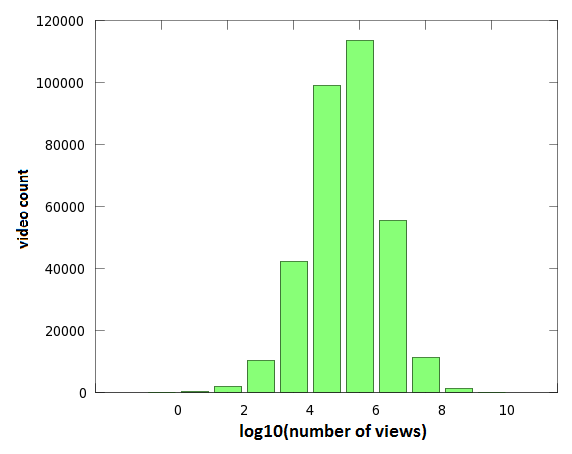
\includegraphics[width=.75\textwidth,clip]{DistributionOfViews.png}
\end{center}

\section{First Steps Taken}

The data gathering required significant time, and is a big part of the project, but apart from this we had to change most of our plans regarding first steps.  Therefore, what we will present in this report is the results of our first attempt to predict the popularity of a video.  For this, we have considered the data from just five days of crawling, and we have reduced the number of fields considered to the title, uploader, video length, and upload date.  We consider only the number-predicting version, not the direct-comparison-prediction version.

\subsection{Technique Details}

We perform  a linear regression on the log of the number of views ("Y") and some features extracted from our video data ("X"), to find the best \beta for Y  = \beta * X.  We also use the log of the number of views as our loss function, rather than using the number of views directly.

The first step is to build a dictionary mapping the uploader to the number of videos they have uploaded and the total number of views there videos have. We also take care to prevent "cheating":  In order to ensure that our predictor has only such information as would be abailiable before the video's publishing is ever used, we temporarily reduce thse number of video-views and the total number of video uploads for the uploader according to the publish date of the video under current consideration.

We train a linear regression model for each of our three outputs on the following features:
\begin{itemize}
\item
Many features extracted via a bag-of-words model on the title, using Tf-idf.
\item
The \# of videos uploaded by the uploader prior to the current video's upload date.
\item
The total \# of views for an uploader due to videos released prior to the current video's upload date.
\item
The fraction of the previous two features (the average number of views per video for videos uploaded by the same uploader prior to the current video's upload date).
\item
The runtime of the video, in seconds.
\item
The age of the video at the time of crawling, in days.
\end{itemize}

We then randomly select 80% of our data for training, and reserve the other 20% for testing.  Once the training is finished, we run the other 20% of our data into the trained model, and consider how much loss was observed.

\section{Results}

\section{Next Steps}

\section{Related work}

\end{document}
